\documentclass[../../thesis.tex]{subfiles}

\graphicspath{{Figures/}}

\begin{document}
\chapter*{Introduction}


% Part 1
Modern cosmology is based on the $\Lambda$CDM model, which predicts the existence of an early phase of exponential expansion of the Universe known as Inflation. This phase plays a central role in our understanding of cosmology, as it is deeply connected to the formation and evolution of the Universe. However, no direct observational evidence supporting this hypothesis has yet been obtained. Consequently, a major goal of current cosmological experiments is to search for such evidence. In particular, efforts are focused on detecting primordial polarisation B-modes patterns in the Cosmic Microwave Background. These patterns are expected to be generated by primordial gravitational waves predicted by inflationary theory. At present, only upper limits on the amplitude of this signal have been established from observations. These elements are introduced and discussed in Chapter~\ref{chap:cosmo}.

% Part 2
The lack of detection is mainly due to the significant challenges associated with these observations. First, the amplitude of primordial B-modes is theoretically expected to be extremely tiny, close to or below the sensitivity of previous experiments as current experiments begin to approach this level. Second, the signal is contaminated by several sources, including astrophysical foregrounds, gravitational lensing, and atmospheric emissions for ground-based missions. Future generations of experiments must therefore achieve precise control of systematic effects while enabling efficient separation between the primordial signal and its contaminants. These considerations motivate the QUBIC experiment, presented in Chapter~\ref{chap:BI}, which is based on bolometric interferometry, an innovative design combining the high sensitivity of bolometers with the unique advantages of interferometry. Interferometry provides a powerful tool for systematic control through self-calibration, a technique widely used in radio interferometry. Preliminary studies of this method were conducted using QUBIC's calibration source, and more specifically its associated GPS system, as described in Chapter~\ref{chap:gps}. In addition, spectral imaging allows the physical bandwidth to be divided during data analysis, thereby improving component separation capabilities. Spectral imaging is a central topic of the thesis, and is detailed in Chapter~\ref{chap:spectral_imaging}.

% Part 3
The main objective of this thesis is the development of map-making methods based on spectral imaging. The first algorithm, called Frequency Map-Making and presented in Chapter~\ref{chap:FMM}, reconstructs frequency maps from observational data. Thanks to spectral imaging, multiple maps can be reconstructed within each physical band. A second and improved method, called Component Map-Making, is introduced in Chapter~\ref{chap:CMM}. This algorithm aims at directly reconstructing astrophysical component maps, performing map reconstruction and component separation simultaneously, which naturally exploits the spectral imaging capability. In addition to map reconstruction, separating the primordial CMB signal from astrophysical foregrounds is essential for achieving B-mode detection. Chapter~\ref{chap:xspectrum} is dedicated to this component separation method and cosmological parameter estimation. These approaches are formulated in spherical harmonic space and rely on the angular power spectra of the CMB and astrophysical emissions. Chapter~\ref{chap:qubicsoft} is devoted to the software development of the experiment, which represented a substantial part of the work carried out during this PhD. Chapter~\ref{chap:tod} further improves the realism of the simulation pipeline, which is the central piece of the software framework. This includes the modelling of various instrumental and physical parameters, convolution effects, the incorporation of external data, and hyperparameter optimisation. In Chapter~\ref{chap:NNMM}, an alternative to the forward-modelling formulation of the two algorithms is introduced, providing an approximate solution to the inverse map-making problem using a physically-guided neural network approach, guaranteeing the interpretability and allowing noise estimation. Chapter~\ref{chap:forecast} presents forecasts for the QUBIC instrument. These include comparisons between different sky models and instrumental configurations, as well as between the various algorithms developed throughout this thesis.

% Part 4
While the previous developments focus on improving map-making and component separation through spectral imaging, they are also applied to a major challenge for ground-based experiments: atmospheric contamination. Traditional strategies rely on data filtering techniques and hardware solutions to reduce atmospheric effects. In contrast, we propose an innovative approach that models the atmosphere as an additional component, evolving in a different domain from astrophysical signals. Chapter~\ref{chap:atm} details this work, from the development of atmospheric simulations to the mitigation of atmospheric contributions in the data using the Component Map-Making algorithm, and compares the results with those obtained using standard filtering methods.

\begin{figure}
    \centering
    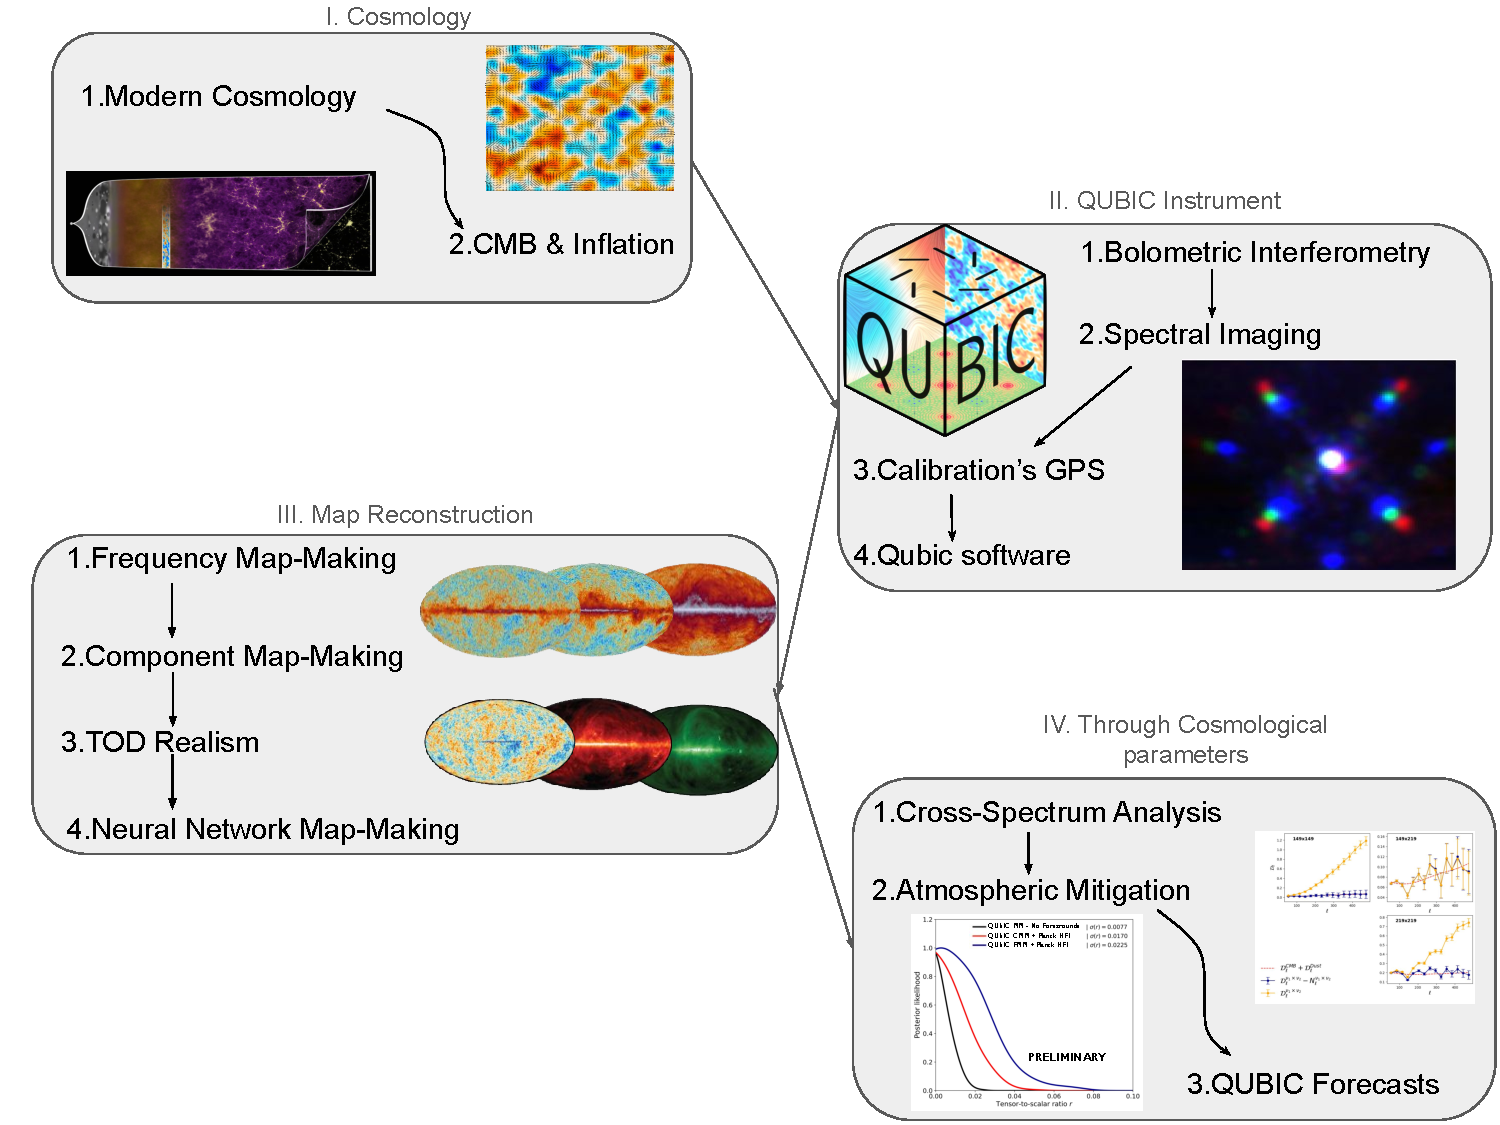
\includegraphics[scale=0.6]{Illustration_intro.pdf}
    \caption{Illustration of the manuscript, showing the different Parts and Chapters.}
    \label{fig:scheme_intro}
\end{figure}

\end{document}